\section{The URDAD metamodel \label{sec:metamodel}}

The URDAD metamodel was developed to provide a formal description of the URDAD domain of discourse that can be efficiently used to support the URDAD methodology for requirements specification. A metamodel is the ``logical information model that specifies the modelling elements used within another (or the same) modelling notation'' \cite{_ieee_2003}. The URDAD metamodel formalizes the modelling constructs needed for the specification of service requirements and the technology neutral design of business processes realizing these requirements\footnote{In the URDAD DSL, the metamodel described in this section, is supplemented with a library of primitive data types, entities, and core persistence services.}. 

The URDAD metamodel was encoded using the EMOF/Ecore \cite{} toolsuite, which provides for 1) the automatic generation of concrete textual and diagrammatic syntaxes, 2) QVT-based model-to-model and model-to-text transformations, and 2) the integrated use of the Object Constraint Language (OCL) \cite{_object_2010} with URDAD (meta-)models. An automatic translation of the metamodel into a Web Ontology Language (OWL DL) \cite{} ontology was employed to facilitate automated satisfiability checking (see Section \ref{sec:assessment}).

The URDAD metamodel was designed to contain the smallest sufficient set of concepts that describe URDAD's services oriented analysis and design. In particular, the described modelling constructs facilitate 1) the recursive decomposition of service requirements into lower level service requirements with pre- and post-conditions, 2) the specification of quality requirements for services, 3) the specification of input/output data structures, and 3) the specification of service orchestrations.

The URDAD metamodel has been influenced by the Unified Modeling Language (UML) and the Business Process Execution Language (BPEL) in the area of data structure specification and process specification, respectively. It enforces the assembly of stateless services from lower level stateless services, where lowest level services are sourced from the environment (see Section \ref{sec:urdadMethodology}). 

The URDAD DSL is only a fraction of the size of UML, yet it includes important core concepts required by the URDAD methodology. In particular, these include 1) a higher-level constraint infrastructure supporting parameterized, reusable constraints, which are assessed through processes that gather information from the environment, 2) modelling constructs for the explicit specification of a service contract, 3) concept relationships facilitating improved traceability, 4) the concept of a responsibility domain, 5) the explicit relation of pre-conditions with exceptions, 6) the separation of the identification of a resource (object or service) from the path to it, and 7) service-specific request and result classes.

%--------------------------

\subsection{URDAD-DSL core}

The core module introduces the concept of an URDAD model, model elements and stakeholders, responsibility domains, and expressions and annotations as shown in Fig.\ \ref{fig:metamodel}. Note that the URDAD-DSL does not lock into a particular expression language (e.g., for the specification of constraints). 

\begin{figure}[Htb]
  \centering
  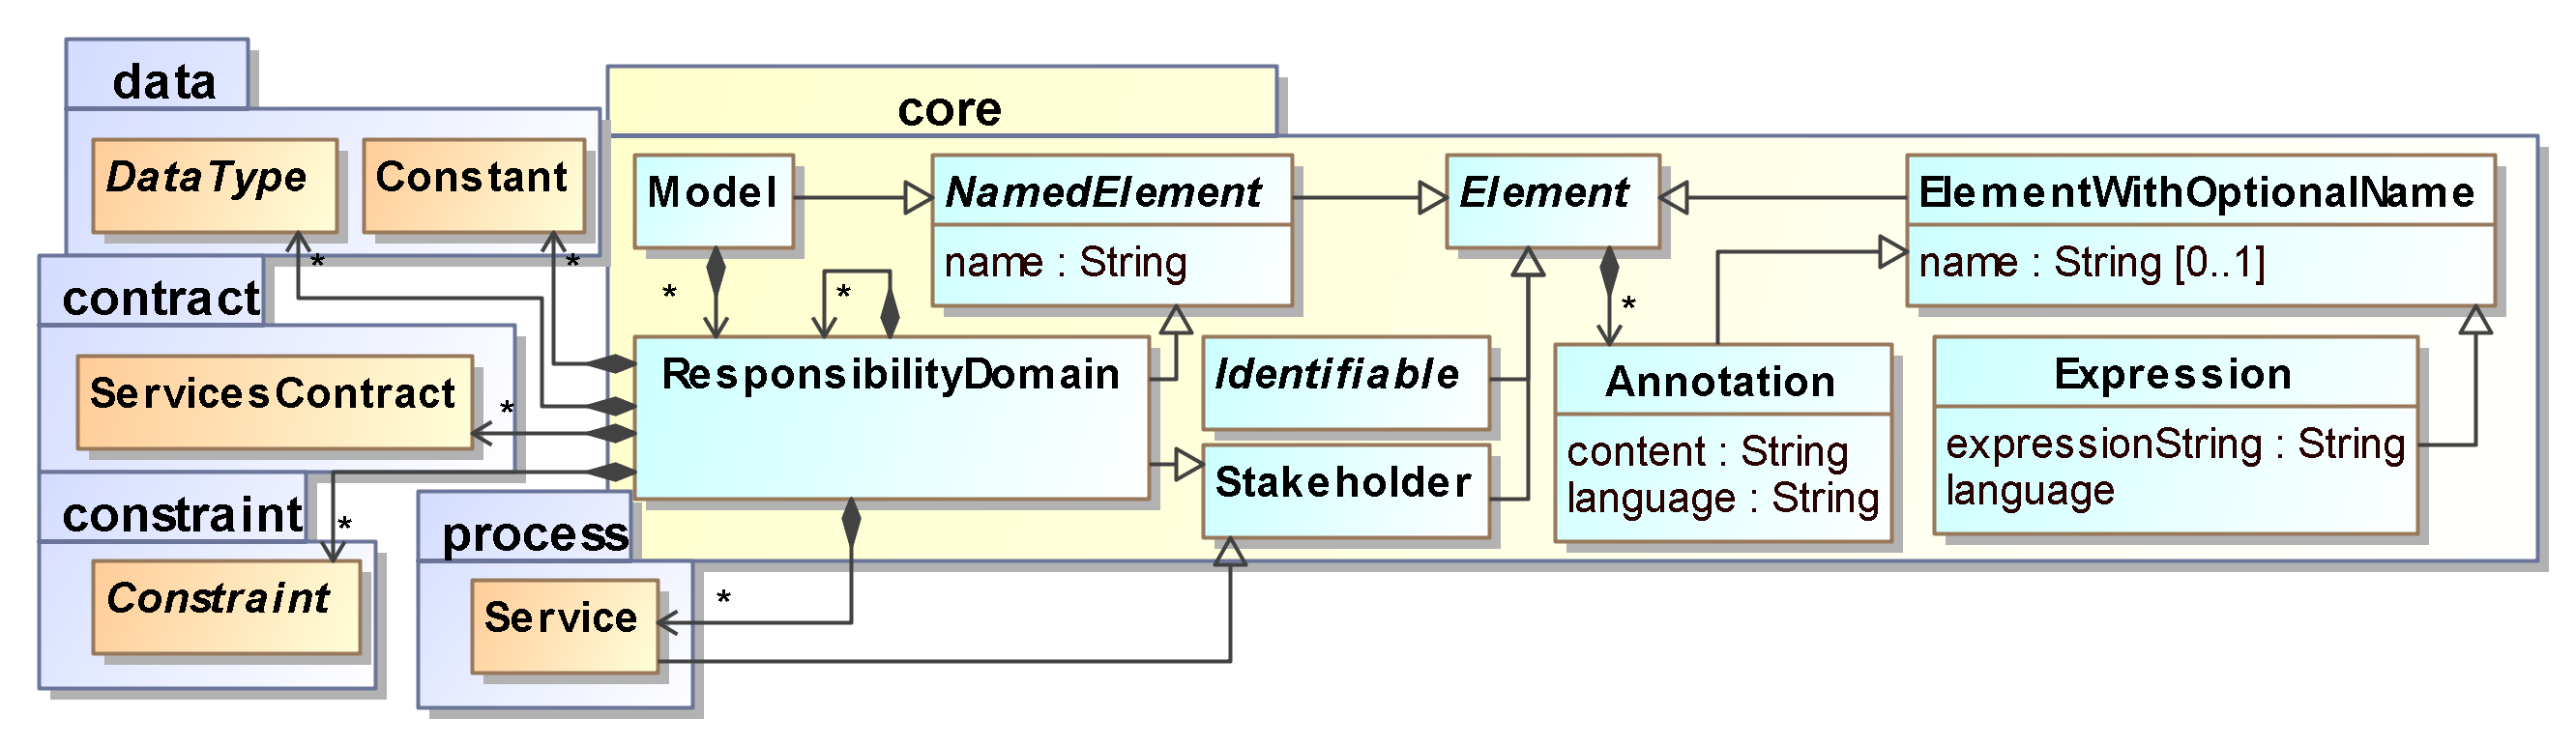
\includegraphics{core}
  \caption{The core elements of URDAD}
  \label{fig:metamodel}
\end{figure}

Responsibility domains are assigned to physical resources (e.g., persons, systems, modules). A responsibility domain covers a cohesive unit of functionality at a particular level of granularity. For example, there may be a finance responsibility and within it there are lower level responsibility domains such as creditors and debtors. Responsibility domains group cohesive service contracts. They define the boundaries between levels of granularity with lower level granularity services of a responsibility domain being contained in lower level responsibility domains. Technically, responsibility domains are packaging constructs associating model elements with a unique namespace. In URDAD, every requirement needs to justified by at least one stakeholder, which can either be a service or a responsibility domain.\todo{I tried to make sense of this paragraph an rephrased it. Please check.}

Responsibility domains are closely related to the concept of unity criteria \cite{gonzalez_unity_2009}.\todo{Move last sentence to Related Work section}

%--------------------------

\subsection{Constraints}

The Object-Constraint Language (OCL) has become the de-facto standard for specifying constraints across object graphs. However, in a services oriented approach and in the context of reusable, parameterized constraints OCL alone is insufficient. In particular, the definition of reusable constraints requires support for binding parameters. Assume, for example, a constraint that a \emph{Person} is registered. This constraint can be used in a pre- and post-condition of a service. Hence, to be able to do so, the person identifier would have to be passed as a parameter to the constraint.

Another reason why the URDAD-DSL provides for the integration of additional constraint infrastructure is that in a services oriented world the actual environmental state is not directly specified, but accessible only via services. In such a world it is not possible to specify testable constraints via a pure\todo{What is the meaning of ``pure'' in this context?} constraint language like OCL. The constraint specification needs to include the specification of services, which are used to obtain the state information and the associated service request objects. The construction of these request objects might itself require a process, which obtains information from the environment. URDAD-DSL constraint specifications include the specification of a process to source information from the environment together with a set of constraints that apply to this information. OCL (or different constraint specification languages) can then be used to specify the constraints that apply to the obtained information.

\begin{figure}[Htbp]
  \centering
  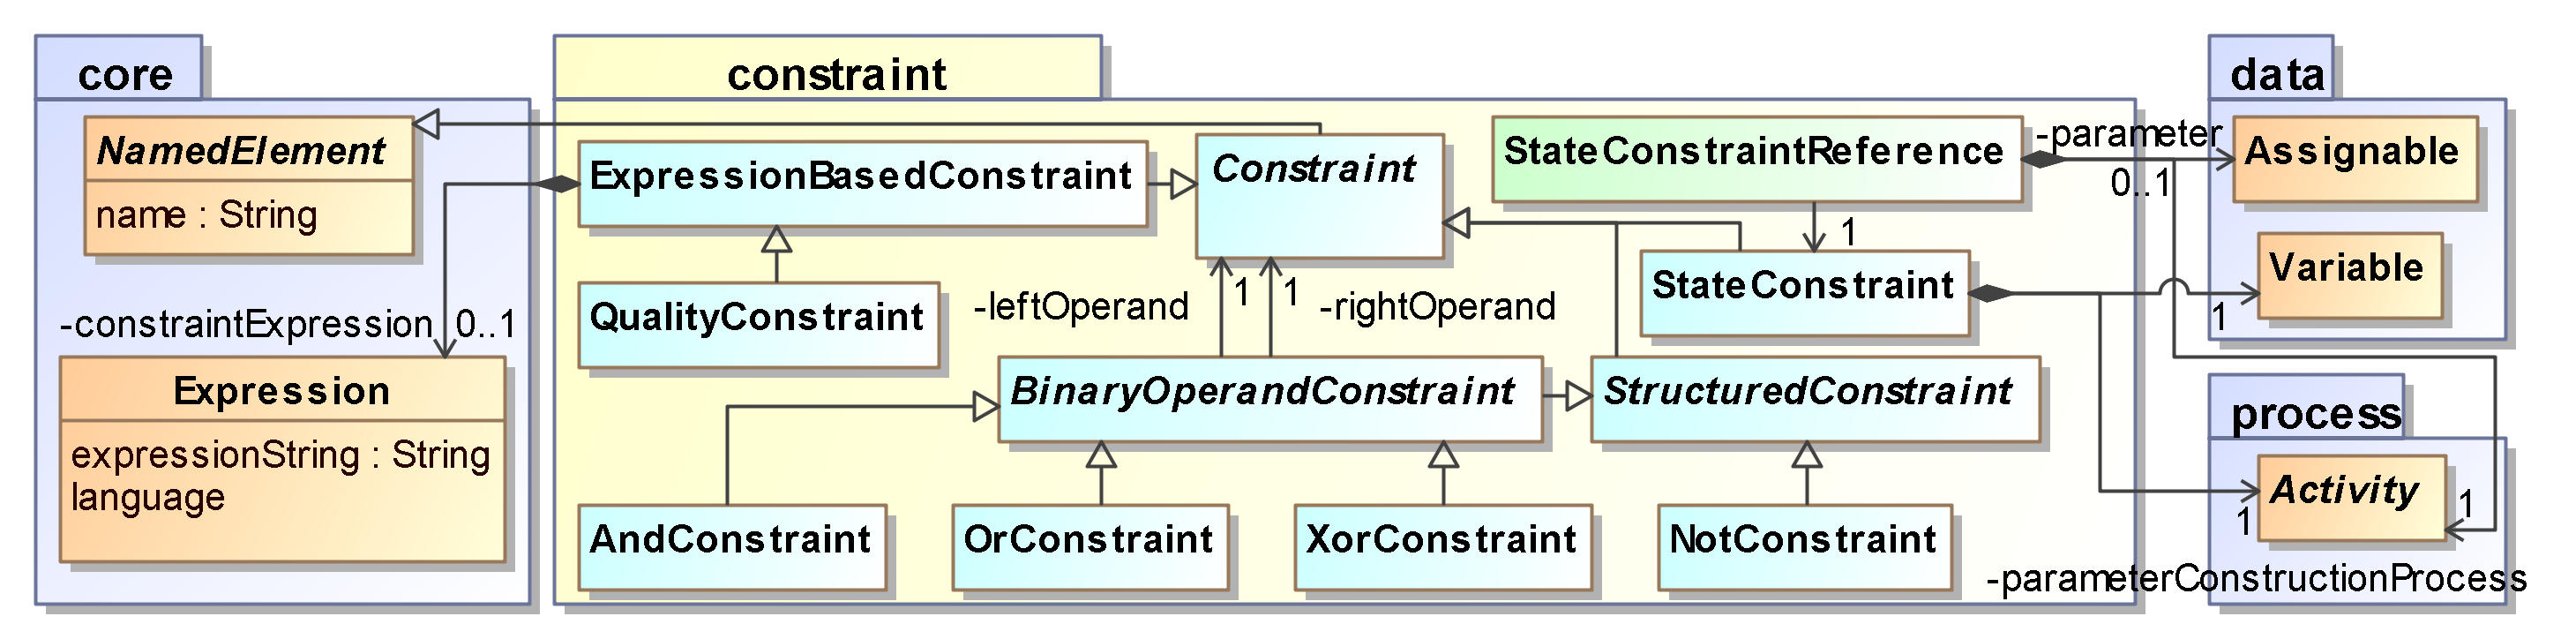
\includegraphics{constraint}
  \caption{The constraint specification elements of URDAD}
  \label{fig:metamodel}
\end{figure}

The constraints module provides the concept of re-usable constraints and standard logical operators to build up complex constraint expressions. Parameterized state constraints are assembled from a process querying the environment and a set of constraints on the information obtained from the environment. A state constraint reference has the option to include a constraint parameter as well as the specification of a process to construct that parameter.

%--------------------------

\subsection{Services contracts}

A service contract can comprise both functional requirements (i.e.\ pre- and post-conditions) as well as non-functional (i.e.\ quality) requirements. Each requirement is associated with a a stakeholder which is either a responsibility domain or another service. 

Pre-conditions are conditions that must be true for a service to execute. Service providers may refuse  services without breaching the service contract if a pre-condition does not hold. In URDAD, the specification of a pre-condition includes the specification of an exception that is used to notify a service user if a requested service cannot be provided (because the pre-condition does not hold). 

A post-condition is a condition that holds true after a service has been provided. It is either a condition of the result or constrains the state of the environment. Due to a service potentially resulting in a lasting change to its environment, the URDAD-DSL allows the designation of inverse services through which these lasting effects can be reversed. Thus, the effects of partially completed processes can be reversed.

Functional requirements may be conditional and are bound to reusable state constraints.  Quality requirements are bound to quality constraints.\todo{Meaning?}

\begin{figure}[Htbp]
  \centering
  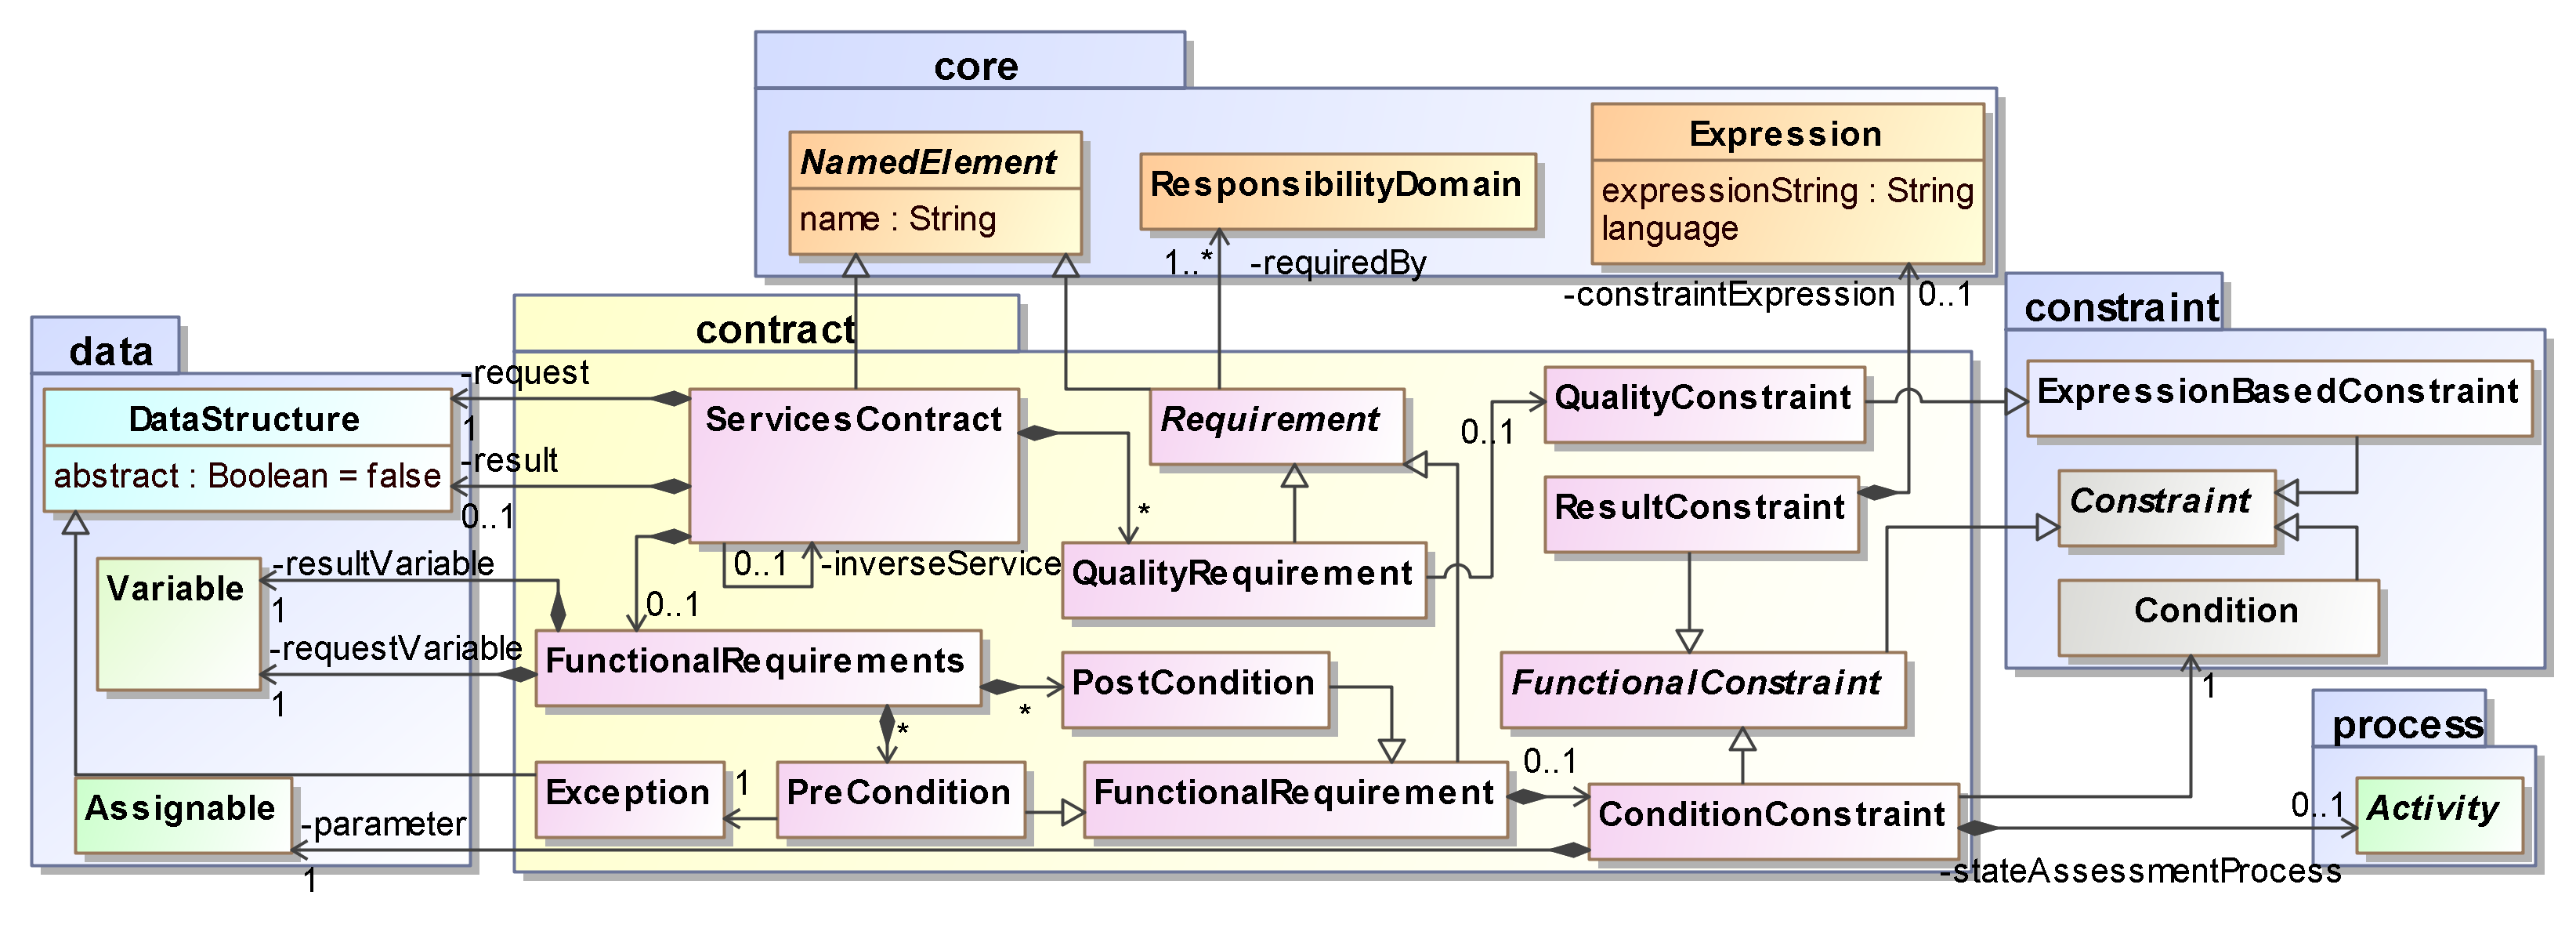
\includegraphics{contract}
  \caption{The contract specification elements of URDAD}
  \label{fig:metamodel}
\end{figure}

A services contract specifies a single service request object that contains information pertaining to the request and a single result object, which comprises of the information associated with the result of the executed service. The data structures for these request and result objects are service specific and are not meant to be reused (their components, which are domain objects, are most likely to be reused).

%--------------------------

\begin{figure}[Htbp]
  \centering
  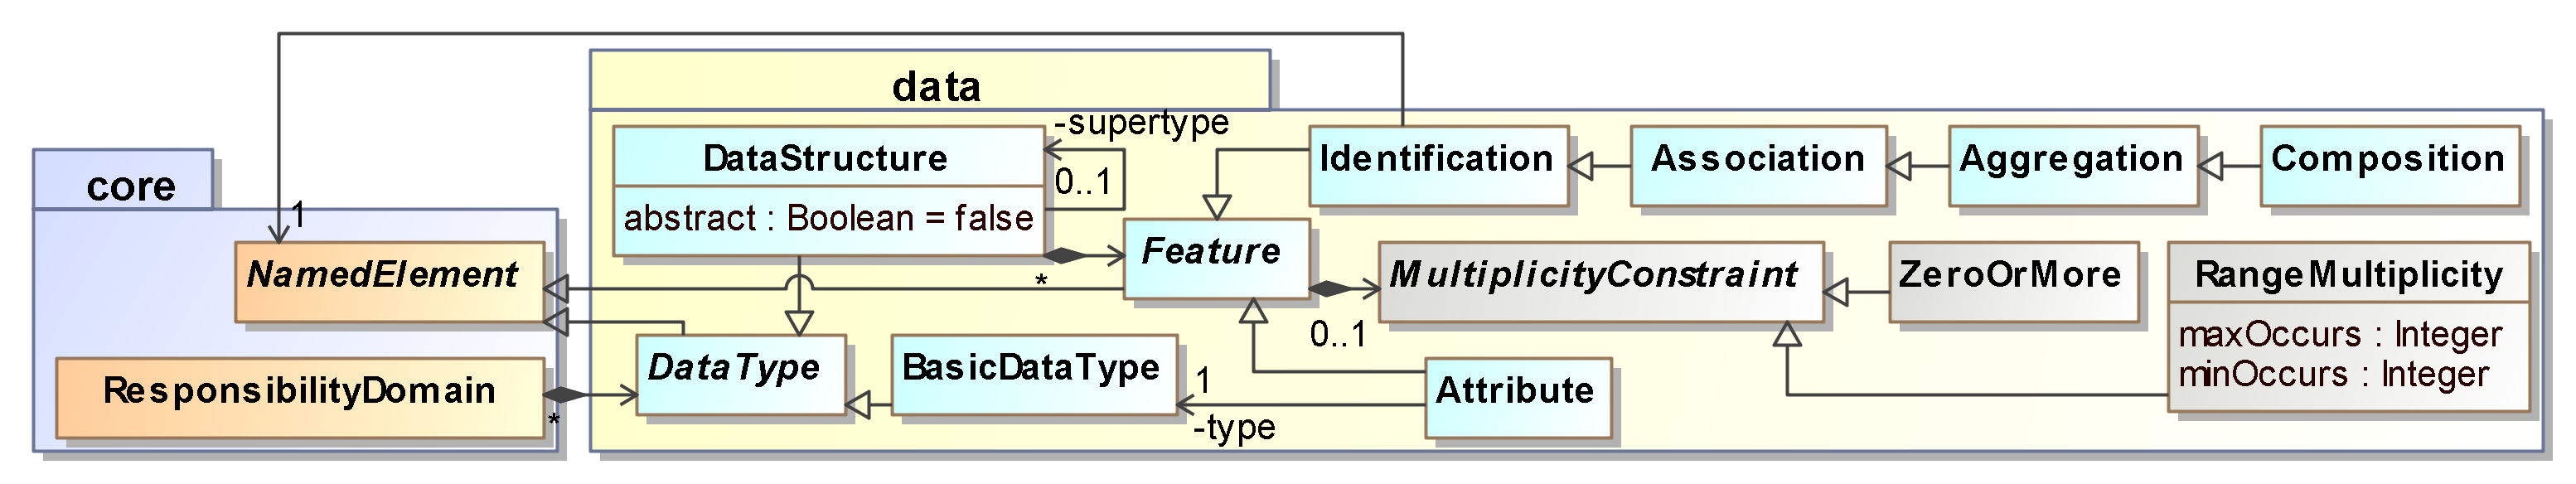
\includegraphics{data}
  \caption{The data definition elements of URDAD}
  \label{fig:metamodel}
\end{figure}

\subsection{Data structures}

The data module of the URDAD metamodel is a straightforward object-oriented approach to data structure specification similar to UML class models. The core additions are that of separating an identification from an association and the concept of an assignable which can be a variable (object), variable reference, query or constant. An identification purely identifies a resource (object or service), relying on the environment to be able to source the resource from the environment. It is an abstraction of the concept of a \emph{Uniform Resource Identifier} (URI). An association, on the other hand, resembles a path to the resource.\todo{Never mind, this paragraph is unintelligible.}

%--------------------------
\begin{figure}[Htbp]
  \centering
  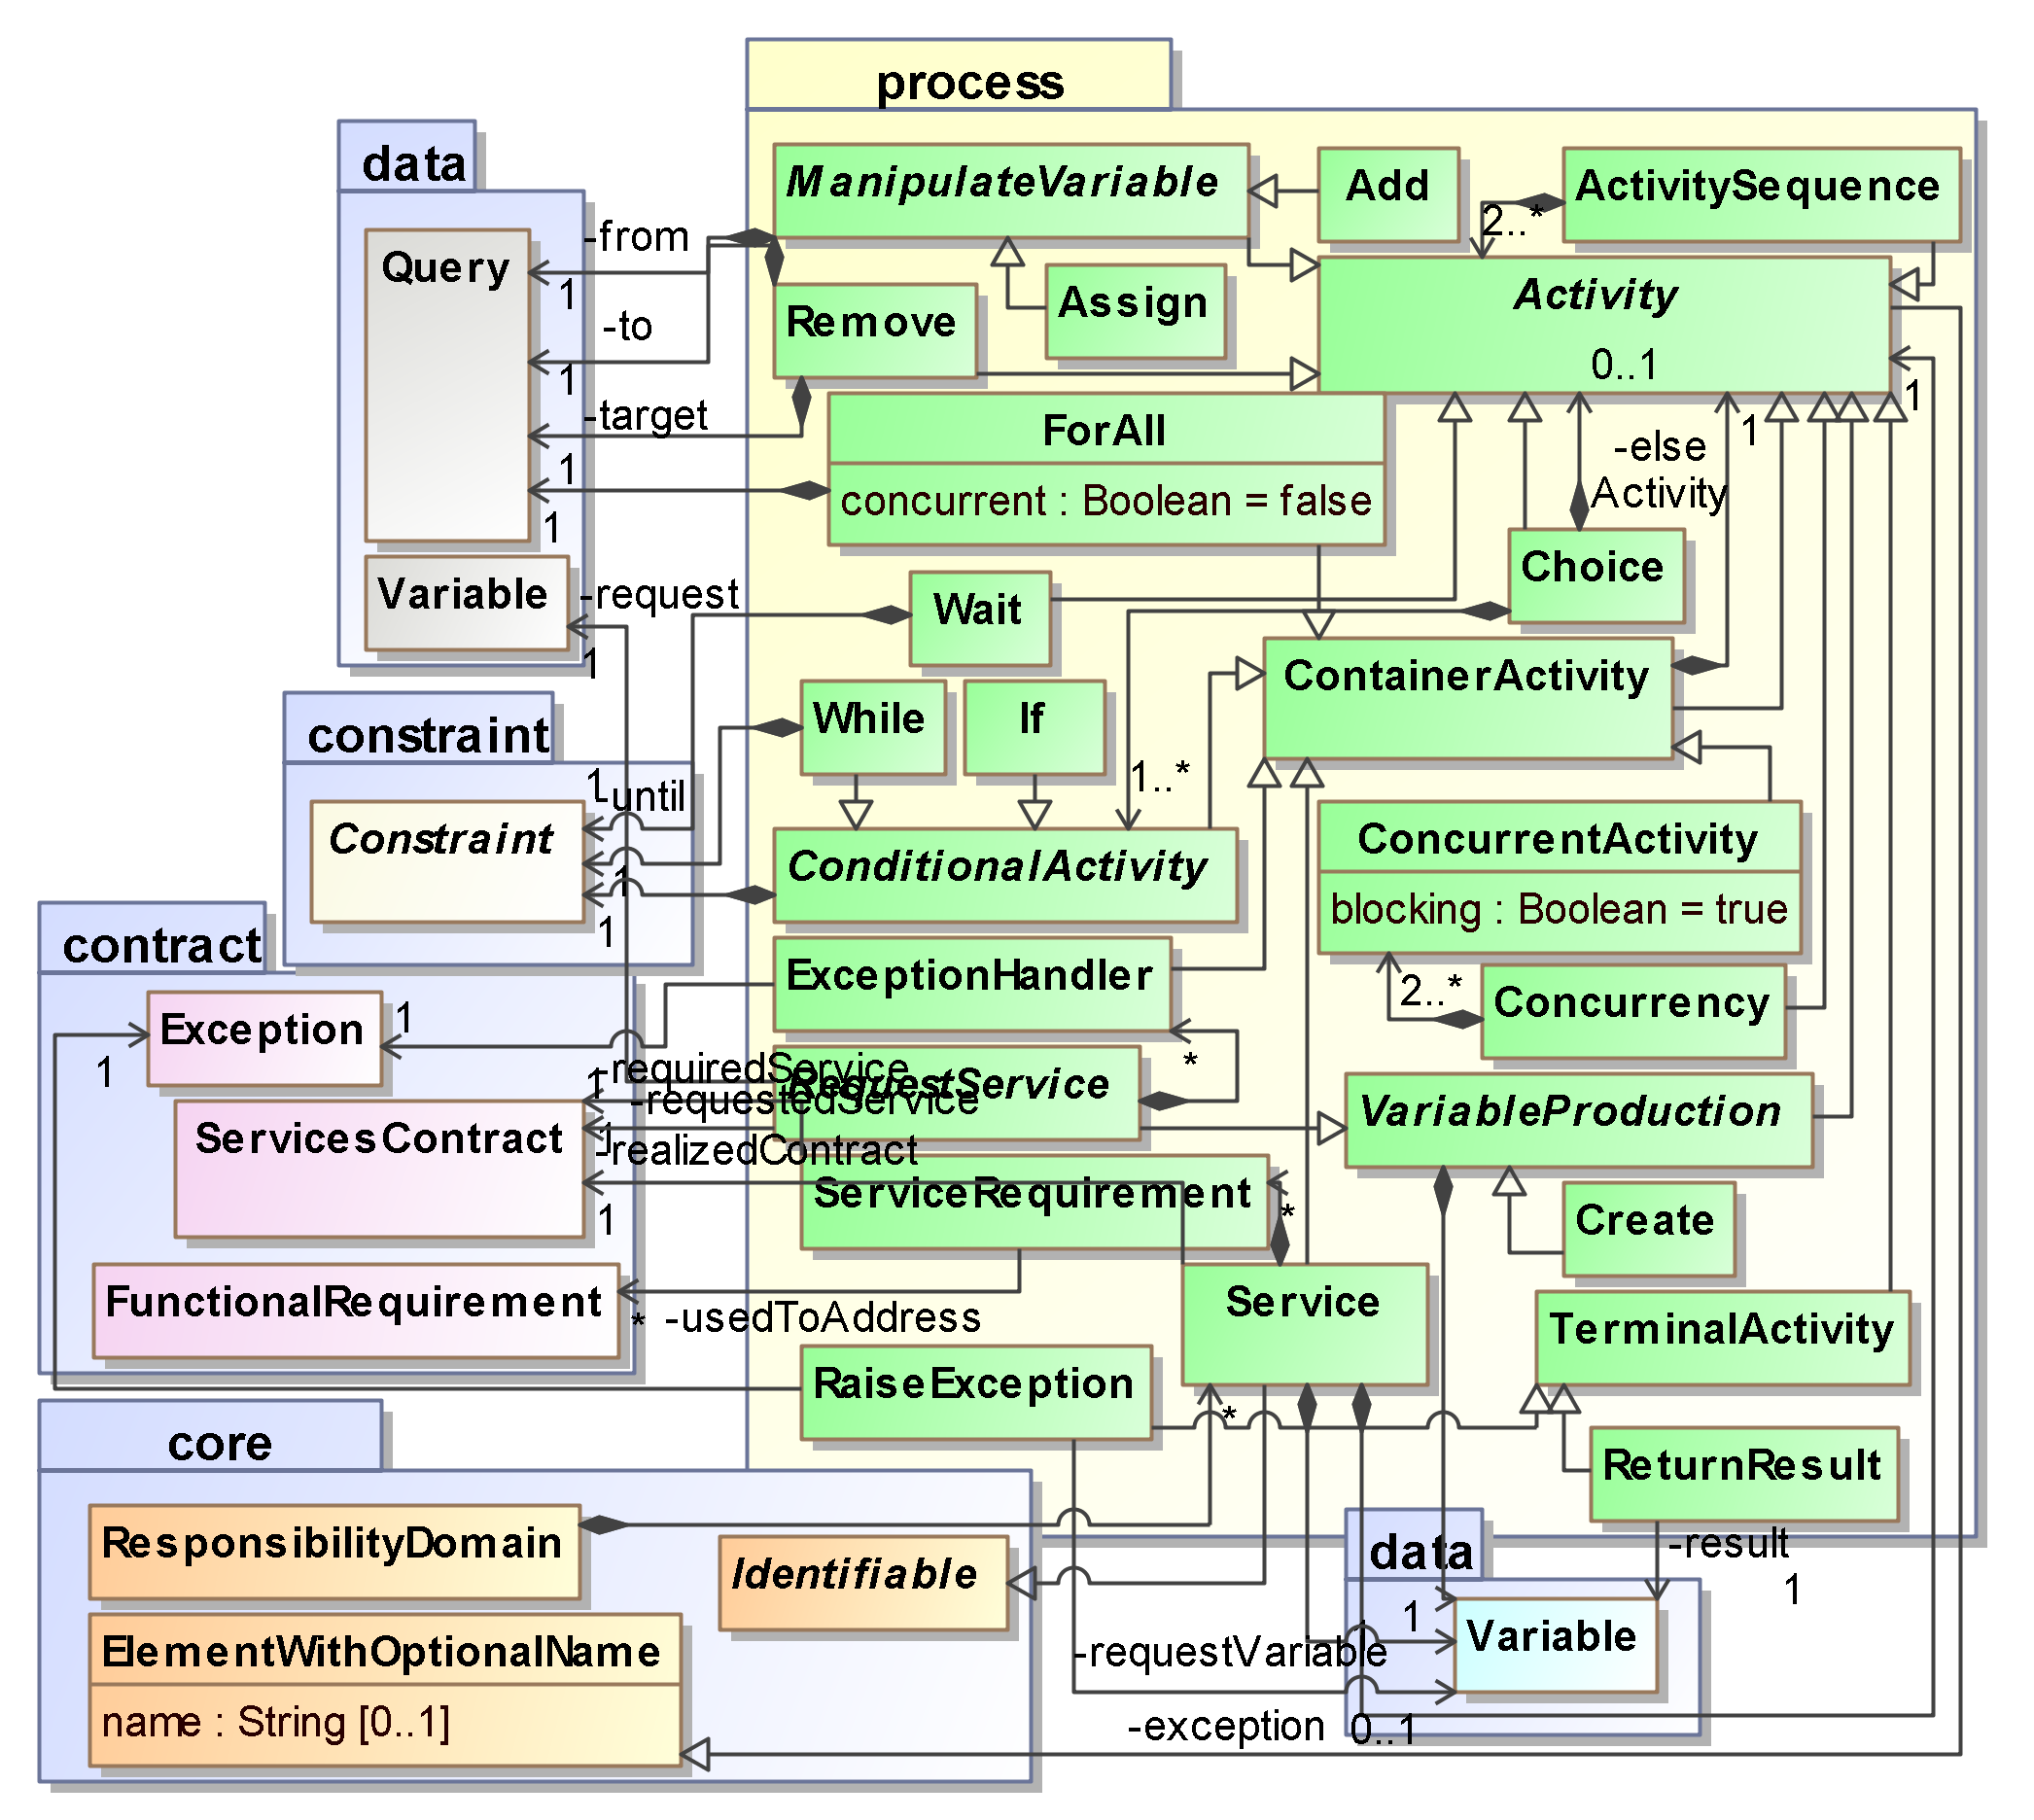
\includegraphics{process}
  \caption{The process definition elements of URDAD}
  \label{fig:metamodel}
\end{figure}

\subsection{Processes}

The process package introduces the concept of a service as a concrete unit of functionality realizing a services contract. A service specification comprises of lower level services used to address stipulated pre- and post-conditions. Thus, the URDAD methodology improves traceability by providing satisfaction links as discussed in \cite{ramesh_toward_2001}). Each activity within the service process is associated with either 1) the maintenance of local process variables\todo{Meaning of item 1)?}, 2) the validation of a pre-condition and/or the fulfilment of a post-condition through the execution of a lower level service, 3) the handling of an exception received from a lower level service, or 4) the raising of an exception or the return of the result.

The URDAD methodology enforces decoupling through services contracts. This is enforced in the URDAD metamodel by linking both satisfaction links as well as service requests to service contracts instead of concrete services. Also note that URDAD assumes that the concrete services used to realize the services contracts are specified either by implementation mapping\todo{Meaning of ``implementation mapping''?} or by the run-time environment and not in the technology neutral model. They could, for example, be injected by the run-time environment similarly to dependency injection on the J2EE platform.

An important non-functional requirement of all activities that constitute a service's process is that each activity must be traceable back to the fulfilment of one or more of the functional requirements. There must be no redundancy and only the functional requirements that are associated with the service must be addressed by a process.